\chapter{Appendiks} \label{cha:AppB}
\section{Udbudstyper ved Amgrosudbud}
Udbudstyper er defineret på forhånd, enten på baggrund af lægemidlets pris, hvilket er tilfældet for de fleste lægemidler, eller ved økonomisk mest fordelagtige udbud, hvor prisen vægtes mod andre kriterier~\citep{Amgros2018a}. Disse kriterier er opstillet på baggrund af juridiske grundlag og kan f.eks. omfatte emballage, håndtering af lægemidlet ved administration samt patientsikkerhedsmæssige aspekter. Der kan være én eller flere vindere, hvilket medfører til fire typer af udbudsformer, hvilket fremgår af figur \ref{fig:TypeUdbud}.~\citep{Amgros2018a}

\begin{figure}[H]\centering
	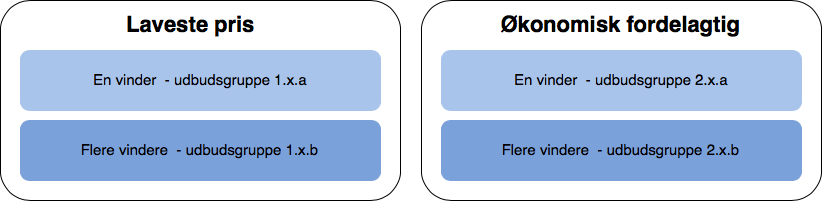
\includegraphics[width=0.7\textwidth]{billeder/TypeUdbud.png} 
	\caption{Udbudstyper inddelt i laveste pris og økonomisk fordelagtig. Tallene 1 og 2 angiver om der er én eller flere vindere, hvor bogstaverne a og b angiver én rammeaftale eller flere parallelle rammeaftaler. ~\citep{Amgros2018a}}
	\label{fig:TypeUdbud}  
\end{figure}

Hvis der er udbud af samme ATC-kode i flere udbudsgrupper vurderes det på baggrund af ATC-kodens årlige omsætning, hvorvidt lægemidlet  skal udbydes som et EU-udbud eller bagatelaftale(BA). EU-udbud sker hvis Apotekets Indkøbspris (AIP) er over 500.0000 kr. årligt og BA sker ved AIP under 500.000 kr. årligt. 

%*** SKAL OMSKRIVES \\
%Et EU-udbud af en ATC-kode dækker samtlige identikationer, hvilket betyder at tilbudsprisen vil være den samme for et lægemiddel uanset hvilken indikation det ordineres til, dette kan betyde at forskellige dispensionsformer og styrker af en given ATC-kode kan være udbudt i forskellige udbudsgrupper. 
%****
%
%\section{Typer af lægemiddelskift}
%Lægemiddelskift kan forekomme i forbindelse med kontraktskift, bagatelkøb eller restordre~\citep{Amgros2015}. Kontraktskift kan forekomme ved at lægemidlerne sendes i udbud, såkaldt amgrosudbud. Udbuddene forekommer hvis der findes mere end én leverandør af lægemidlet. Lægemidlerne bringes derved i konkurrence, hvilket kan give anledning til kontraktskift. I tilfælde af patent på lægemidlet, hvormed der kun findes én leverandør, er der ofte ikke konkurrence, da prisen på lægemidlet allerede er fastsat.~\citep{Amgros2015} 
%
%En gang årligt omkring maj eller juni publiceres bagatelkøb af Amgros, hvilket kan forårsage lægemiddelskift~\citep{Amgros2018}. I disse tilfælde modtager Amgros pristilbud fra leverandørere med henblik på økonomiske besparelser på lægemiddlerne~\citep{Amgros2012}. I disse tilfælde er Sygehusapoteket er ikke forpligtet til at anvende lægemidlet og leverandøren omfattes ikke af indkøbs- eller forsyningspligt, som ved kontraktskift.~\citep{Amgros2018}
%
%Restordre forekommer når efterspørgslen på et lægemiddel overstiger den tilgængelige mængde.~\citep{Amgros2015}. Dette kan f.eks. ske ved leveringesvigt fra leverandøren eller producenten på det ønskede lægemiddel~\citep{Amgros2017, Laegemiddelinformaion2017}. Leveringesvigt skyldes som ofte at producenten har mangel på råvarer eller produktionsvanskeligheder~\citep{Amgros2017, Laegemiddelinformaion2017}. I tilfælde  af restordre er det leverandørens ansvar at dække hospitalsapotekernes udgift ved indkøb af et erstatningslægemiddel\fxnote{KILDE}.